\documentclass[12pt,english]{article}
\usepackage[utf8]{inputenc}
\usepackage[a4paper]{geometry}
\geometry{verbose,tmargin=2cm,bmargin=2cm,lmargin=3cm,rmargin=2cm,headheight=12pt,headsep=24pt}
\setcounter{secnumdepth}{3}
\setcounter{tocdepth}{3}
\usepackage{pdfpages}
\usepackage{bm}
\usepackage{array}
\usepackage{float}
\usepackage{graphicx}
\usepackage{tocloft}
\usepackage{hyperref}
\hypersetup{
    colorlinks=true,
    linkcolor=blue,
    filecolor=blue,      
    urlcolor=blue,
}
\usepackage{setspace}
\PassOptionsToPackage{normalem}{ulem}
\usepackage{ulem}
\usepackage{indentfirst}	%Az összes címsor utáni bekezdést beljebb viszi%
\usepackage{amsmath}
\usepackage{tikz}
\usepackage{wrapfig}
\usetikzlibrary{shadings}

\usepackage{pgfplots}


\usepackage{hyperref}
\hypersetup{
    colorlinks,
    citecolor=black,
    filecolor=black,
    linkcolor=black,
    urlcolor=black
}




\makeatletter

%%%%%%%%%%%%%%%%%%%%%%%%%%%%%% LyX specific LaTeX commands.
\newcommand{\noun}[1]{\textsc{#1}}
%% Because html converters don't know tabularnewline
\providecommand{\tabularnewline}{\\}

%%%%%%%%%%%%%%%%%%%%%%%%%%%%%% Textclass specific LaTeX commands.
\newenvironment{lyxcode}
{\par\begin{list}{}{
\setlength{\rightmargin}{\leftmargin}
\setlength{\listparindent}{0pt}% needed for AMS classes
\raggedright
\setlength{\itemsep}{0pt}
\setlength{\parsep}{0pt}
\normalfont\ttfamily}%
 \item[]}
{\end{list}}

%%%%%%%%%%%%%%%%%%%%%%%%%%%%%% User specified LaTeX commands.
%\textwidth 160mm
%\oddsidemargin 0cm
%\topmargin -15mm
\usepackage{bm}
\newcommand{\tg}{\mathop\mathrm{tg}}
\newcommand{\grad}{\mathop\mathrm{grad}}
\newcommand{\BME}{\hrule\vspace{6pt}{\large Budapest University of Technology and Economics
\\
Faculty of Mechanical Engineering \\
Department of Applied Mechanics}}
\newcommand{\szerzo}{}
\newcommand{\konzulensek}{
\parbox[t]{20cm}
{\normalsize
\hspace*{25em} Made by:\\
\hspace*{28em}Bálint CSATÓ\\
\hspace*{25em}Supervisor:\\
\hspace*{28em}Gergely GYEBRÓSZKI \\
}\hfill}

\makeatother

\usepackage{babel}


\begin{document}



\title{\vspace{-2cm}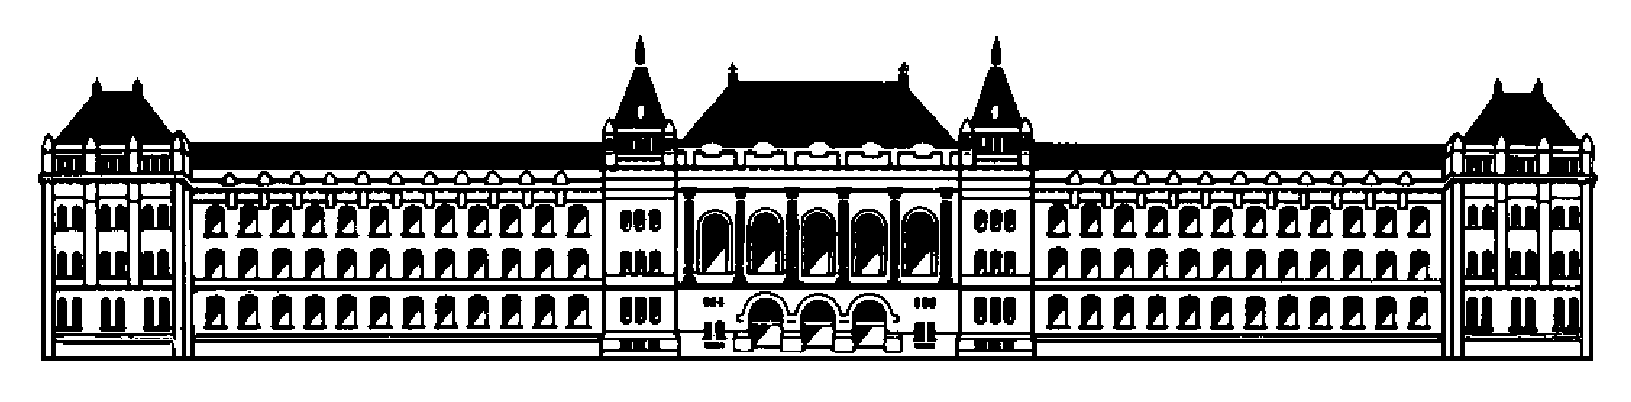
\includegraphics[width=0.4\textwidth,keepaspectratio]{bme_skyline}\\
\BME\vspace{4cm}\\
Control and Parameter Estimation Problems of Autonomous Transport Robots
\\[5mm]
\large{Final Project}}


\author{\sc\szerzo}


\date{\vspace{6cm}\konzulensek\\
\vspace{3cm}Budapest, 2018}

\maketitle
\thispagestyle{empty}



\newpage
\pagenumbering{arabic}
\renewcommand{\contentsname}{Contents}
\renewcommand{\cftsecleader}{\cftdotfill{\cftdotsep}}
\tableofcontents


\newpage

\section*{Preface}
Autonomous vehicle technology offers the possibility of fundamentally
changing transportation. Equipping cars and light vehicles
with this technology will likely reduce crashes, energy consumption,
and pollution and reduce the costs of congestion, as well.

This technology is most easily conceptualized using a five-part
continuum suggested by the National Highway Traffic Safety Administration
(NHTSA), with different benefits of the technology realized
at different levels of automation:
\begin{itemize}
\item \textbf{Level 0:}  The human driver is in complete control of all functions of the car.
\item \textbf{Level 1:}  One function is automated.
\item \textbf{Level 2:}  More than one function is automated at the same time (e.g., steering and acceleration), but the driver must remain constantly attentive.
\item \textbf{Level 3:} The driving functions are sufficiently automated that the driver can safely engage in other activities.
\item \textbf{Level 4:} The car can drive itself without a human driver.
\end{itemize}
\noindent Careful policymaking will be necessary to maximize the social
benefits that this technology will enable, while minimizing the disadvantages[1].


\addcontentsline{toc}{section}{Preface}

\newpage

\section{Autonomous Transport Robots"}





\newpage
\begin{thebibliography}{1}

\addcontentsline{toc}{section}{References}

\bibitem {c} James M. Anderson, Nidhi Kalra, Karlyn D. Stanley, Paul Sorensen, Constantine Samaras, Oluwatobi A. Oluwatola: \emph{Autonomous Vehicle Technology}


\bibitem {c} https://www.hackerearth.com/practice/algorithms/graphs \href{https://www.hackerearth.com/practice/algorithms/graphs/depth-first-search/tutorial/}{[link]}


\bibitem {c} https://www.hackerearth.com/practice/algorithms/greedy \href{https://www.hackerearth.com/practice/algorithms/greedy/basics-of-greedy-algorithms/tutorial/}{[link]}


\bibitem{whatisarduino} Alan G. Smith: \emph{Introduction to Arduino, 2011}


\bibitem{communication_arduino} Brian W. Evans: \emph{Arduino Programming Notebook, 2007}


\bibitem{i2c_communication_arduino} Alex Lange: \emph{I2C Communication with Arduino, 2015}

\bibitem{i2C_communication_arduino_2} http://howtomechatronics.com \href{http://howtomechatronics.com/}{[link]}

	\bibitem{orientation_arduino} Kevin Townsend: \emph{Adafruit BNO055 Absolute Orientation Sensor, 2017}

	\bibitem{optical flow} https://github.com/Lauszus/ADNS3080 \href{https://github.com/Lauszus/ADNS3080}{[link]}
	
	



\end{thebibliography}

\end{document}
